\documentclass[11pt]{article}

% Template-agnostic preamble (works without any venue style file).
\usepackage[margin=1in]{geometry}
\usepackage[utf8]{inputenc}
\usepackage[T1]{fontenc}
\usepackage{hyperref}
\hypersetup{colorlinks=true, linkcolor=blue, citecolor=blue, urlcolor=blue,
  pdftitle={Modality Matters: A Transient Behavioral Interruption Rescues Agent WANDERING Where Residual Steering Does Not}}
% Aggressive spacing to avoid overfull boxes from long dataset/path names.
\emergencystretch=3em
\sloppy
\hyphenpenalty=2000
\exhyphenpenalty=0
\hbadness=10000
\usepackage{booktabs}
\usepackage{amsfonts}
\usepackage{amsmath}
\usepackage{amssymb}
\usepackage{xcolor}
\usepackage{array}
\usepackage{graphicx}

\title{Modality Matters: A Transient Behavioral Interruption Rescues \\
Agent WANDERING Where Residual Steering Does Not}

\author{Anonymous Authors\\\textit{(submitted for double-blind review)}}

\begin{document}

\maketitle

\begin{abstract}
A multi-turn coding agent fails in a distinctive way we call \textbf{WANDERING}: it keeps acting --- reading, editing, running commands --- but never emits the \texttt{finish} action, exhausting its turn budget. A companion line of work detects WANDERING from a residual-stream signature and a probe-free tool-entropy signal, but three pre-registered attempts to \emph{intervene} on the residual stream (injecting a SUCCESS-direction at the output layer L55 and at the locus L11 that best discriminates WANDERING) all fail to rescue it. We ask whether the missing lever is not the locus but the \emph{modality}. On the same 20 WANDERING Qwen3.6-27B SWE-bench Pro trajectories, gated by the same live tool-entropy collapse detector, we contrast four interventions that differ only in modality: no intervention; residual L11 injection; a content-neutral message; and a behavioral re-plan message. Analyzed paired (mandatory under run-instability), the behavioral interruption \textbf{roughly doubles the finalization rate, $30\% \to 70\%$ (McNemar $p=0.021$)}, while residual injection is inert ($40\%$ vs.\ $30\%$, $p=0.63$). Crucially the lever is the \emph{interruption, not its content}: a neutral message that explicitly tells the agent to keep going rescues exactly as well as the re-plan message (B0 $\equiv$ B1, $p=1.0$). SWE-bench Pro Docker evaluation indicates the rescued finalizations are real fixes and that the interruption also raises the task solve-rate ($\sim$23\% $\to$ 50\%, paired $5$--$0$, $p=0.062$, cross-session) --- a suggestive secondary effect. The result completes a four-paper arc (detect $\to$ localize $\to$ residual fails $\to$ behavioral works): for long-horizon agents, the predictive signal lives in the residual stream but the causal lever lives in behavior.
\end{abstract}

\section{Background}\label{sec:background}

\textbf{WANDERING.} Give a capable model a real software issue, a shell, and a fixed turn budget. Most runs end in one of two ways: the agent submits a patch via a \texttt{finish} tool (SUCCESS), or it locks onto a dead end and gives up early (LOCKED). A third failure is quieter: the agent keeps working turn after turn and never decides it is done, exhausting the budget without ever calling \texttt{finish}. We call this WANDERING. It is expensive (the full budget is consumed) and silent (the agent looks busy throughout), which makes it a natural target for monitoring and intervention.

\textbf{The detector, and the mechanism hypothesis.} The Tool-Entropy companion paper \cite{tool_entropy} shows WANDERING is detectable: in its final turns a WANDERING agent's distribution over tool-call names \emph{collapses} (low Shannon entropy), and this signature generalizes across architectures. That paper proposed a mechanism (its \S13): the mid-layer ``verdict'' that the task is done is consolidated, but the edge circuits that translate the verdict into the \texttt{finish} \emph{action} fail to fire --- a decision-to-action desynchronization. The multi-channel classification paper \cite{multichannel} independently localizes the strongest WANDERING discriminator to an early, edge layer (L11) by stability selection.

\textbf{The residual nulls.} If the mechanism is ``mid-layer ready, edge fails to emit,'' the obvious fix is to inject the SUCCESS-typical edge-layer residual into a WANDERING trajectory to supply the missing translation. The residual-intervention paper \cite{residual_nulls} pre-registers and runs exactly this, three times: a forced-finish counterfactual (does WANDERING already secretly succeed? --- no, Fisher $p=0.71$); always-on SUCCESS-donor injection at the output layer L55 (inert, Fisher $p=1.00$); and, re-targeted to L11 --- the layer \cite{multichannel} flags as WANDERING's strongest discriminator --- a norm-matched magnitude sweep. The L11 injection is \emph{not} inert (it destabilizes the model into malformed tool calls at high magnitude) but it does \emph{not} rescue (paired McNemar $p=0.73$). Correcting the locus from L55 to L11 did not convert the null. The conclusion of \cite{residual_nulls} is sharp: the residual signal that \emph{detects} WANDERING is not a residual \emph{lever} that fixes it, even at the strongest detector locus.

\textbf{This paper.} The residual nulls leave one variable unexplored: the intervention \emph{modality}. All three prior attempts perturb the residual stream. Here we hold the locus question fixed (we intervene at the same detector-gated turn) and vary only \emph{how} we intervene --- a residual activation edit versus a behavioral message at the action interface. We ask: is the missing lever behavioral?

\section{Related Work}\label{sec:related}

\textbf{The knowledge-action gap is now consensus --- for single-forward-pass settings.} Basu et al.\ \cite{basu_kag} name the ``knowledge-action gap'': linear probes detect model errors at near-perfect AUROC while four intervention paradigms (concept-bottleneck steering, SAE feature steering, activation patching, task-vector steering) correct almost none of them. Bhalla et al.\ \cite{bhalla_pc} name the ``predict/control discrepancy'': the features that predict a behavior are not the ones that control it. We do not claim the asymmetry as novel; we cite into it. What is unexamined in this literature is the asymmetry \emph{on long-horizon agents}, where the failure is a multi-turn behavioral mode rather than a single-token error, and --- critically --- whether a \emph{behavioral} lever closes the gap the residual lever cannot.

\textbf{Behavioral course-correction of agents.} SWE-PRM \cite{swe_prm} course-corrects looping SWE agents at inference time with a process reward model, and its failure taxonomy (redundant exploration, looping, failure to terminate) overlaps WANDERING; it establishes that \emph{behavioral} intervention can rescue looping agents. Our contribution is not behavioral-rescue per se --- it is the controlled \emph{modality contrast}: behavioral rescue \emph{where residual injection fails}, on the same trajectories at the same trigger, plus the finding that the rescue is the interruption and not its content. SafeThink \cite{safethink} shows a transient early intervention suffices for safety recovery (a structural analog, but activation-based and not agent-failure). EAST \cite{east} shows activation steering \emph{can} move an agent's exploration entropy --- so our residual null is specifically about \emph{finalizing}, not about whether activations move agent behavior at all. StepShield \cite{stepshield} formalizes the ``intervention gap'' (time from first problematic behavior to intervention) that our detector-gated design optimizes. The tool-entropy signal we trigger on is independently validated as a model-agnostic quality signal \cite{tool_entropy_train}. The nearest method-competitor reads pre-action agent activations to predict tool need/risk but is detection-only and does not steer \cite{tatsat}. Our own prior work supplies the detector \cite{tool_entropy}, the localization \cite{multichannel}, and the residual nulls \cite{residual_nulls}.

\section{Method}\label{sec:method}

\textbf{Population.} The 20 WANDERING trajectories from \cite{residual_nulls,multichannel}: Qwen3.6-27B on SWE-bench Pro, 50-turn budget, temperature 1.0, captured at L11/L23/L31/L43/L55. All runs use the deterministic per-instance seed. Hardware: one RTX 6000 Pro Blackwell (96 GB).

\textbf{Live trigger.} We fire one intervention per trajectory, online, at the first turn $\geq 10$ at which the Shannon entropy of the last-10 tool-call names drops below $\tau=0.503$ --- the operating threshold of the deployed v5 detector \cite{tool_entropy}. Computed from the running trajectory's own tool history (no oracle), the trigger fires on 18 of 20 instances in the live runs (19/20 in calibration on the original no-hook traces) at a median turn of 17, leaving roughly 30 turns for the intervention to act. This mimics deployment: the detector flags the collapse, and we intervene.

\textbf{Four arms, varied only in modality.} At the trigger turn we apply one of:
\begin{itemize}
\item \textbf{Arm 0} --- nothing (no-intervention baseline).
\item \textbf{Arm A (residual)} --- attach a SUCCESS-donor injection at L11, $\alpha=0.70$, \texttt{mode=add}, for the remaining turns (the lever of \cite{residual_nulls}, here detector-gated).
\item \textbf{Arm B0 (behavioral, neutral)} --- inject one \texttt{user} message of matched length with content-neutral text: \emph{``Here is a brief checkpoint note for your records. You may continue working on the task as you see fit; no change of approach is required. Proceed with whatever next step you judge appropriate.''}
\item \textbf{Arm B1 (behavioral, re-plan)} --- inject one \texttt{user} message: \emph{``You appear to be repeating similar tool calls without converging. Stop and re-plan: in 2--3 sentences state what you have already established, then either (a) call finish\_tool with your best patch now, or (b) name the single concrete blocker and the one next action to resolve it.''}
\end{itemize}
B0 is the behavioral analog of a placebo: it controls for ``a message appeared / the context was refreshed / a turn was consumed,'' isolating the re-plan \emph{content}. All four arms run in the same session with the same seeds, so they share the pre-trigger trajectory and diverge only at the intervention.

\textbf{Analysis: paired, never definitional.} WANDERING is not run-stable under temperature sampling (\cite{residual_nulls}: the same 20 instances flip \texttt{finish} $\sim$35\% on a no-hook re-run). The only valid finalization test is therefore paired against the same-session Arm 0 (McNemar on discordant pairs), never against the definitional ``0/20 all-WANDERING'' baseline. We pre-register three hypotheses: \textbf{H1} B1 $>$ 0 (does behavioral rescue?), \textbf{H2} B1 $>$ A (does modality matter?), \textbf{H3} B1 $>$ B0 (is it the content?).

\textbf{Solve-rate.} Finalizing is the WANDERING-specific behavior, but a \texttt{finish} on a wrong patch is not a real fix. We therefore also score patch correctness with the official SWE-bench Pro Docker harness (apply the model patch to the base commit in a per-instance image, run the gold FAIL\_TO\_PASS and PASS\_TO\_PASS tests). Patches are computed as \texttt{git diff HEAD} where HEAD already contains the committed gold-test patch, so the scored diff excludes the gold tests (no leakage).

\section{Results}\label{sec:results}

\begin{figure}[t]
\centering
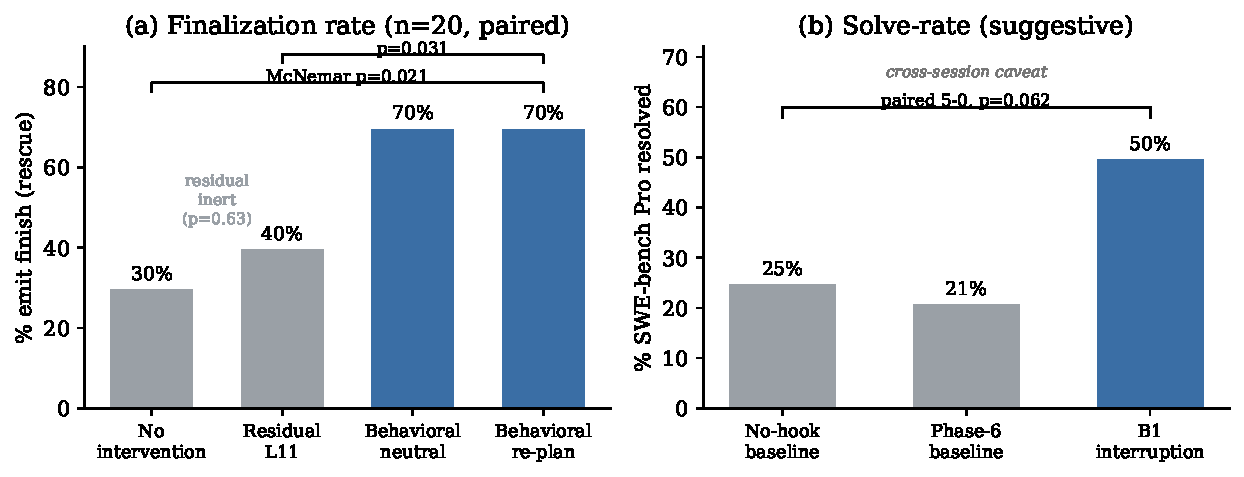
\includegraphics[width=\textwidth]{figures/main_result.pdf}
\caption{\textbf{Modality matters.} (a) Finalization rate by intervention arm on the same 20 WANDERING trajectories, gated by the same live tool-entropy collapse detector. The two behavioral arms (blue) roughly double the rate at which agents emit \texttt{finish} (30\% $\to$ 70\%); the residual L11 injection (gray) is inert ($A$ vs.\ $0$, $p=0.63$). A content-neutral message rescues as well as a re-plan ($B0\equiv B1$, $p=1.0$): it is the interruption, not the content. (b) SWE-bench Pro solve-rate. The behavioral interruption (B1, 50\%) strictly dominates two independent no-intervention baselines ($\sim$23\%; paired $5$--$0$, $p=0.062$) --- a suggestive secondary effect carrying a cross-session caveat (\S\ref{sec:results}).}
\label{fig:main}
\end{figure}

\subsection{Finalization: behavioral rescues, residual is inert}

\begin{center}
\begin{tabular}{lccc}
\toprule
Arm & \texttt{finish} (rescue) & \texttt{max\_turns} & \texttt{invalid\_tools} \\
\midrule
0 --- no intervention & 6/20 (30\%) & 14/20 & 0 \\
A --- residual L11 ($\alpha{=}0.70$) & 8/20 (40\%) & 12/20 & 0 \\
B0 --- behavioral, neutral & 14/20 (70\%) & 6/20 & 0 \\
B1 --- behavioral, re-plan & 14/20 (70\%) & 6/20 & 0 \\
\bottomrule
\end{tabular}
\end{center}

The behavioral arms roughly double the finalization rate (30\% $\to$ 70\%); the residual arm barely moves it (Figure~\ref{fig:main}a). Paired McNemar ($n{=}20$; the $\leq 2$ instances that never trigger receive no intervention and are concordant by construction, so restricting to the triggered subset gives identical discordant counts):
\begin{itemize}
\item \textbf{H1 (B1 vs.\ 0):} 9 B1-only flips vs.\ 1 baseline-only, \textbf{McNemar $p=0.021$ --- PASS.} The behavioral interruption causally increases finalization.
\item \textbf{H2 (B1 vs.\ A):} 6 B1-only vs.\ 0 A-only, $p=0.031$ --- \textbf{PASS}. Modality matters: behavioral beats residual.
\item \textbf{A vs.\ 0:} 3 vs.\ 1, $p=0.63$ --- \textbf{null}. Residual injection does not beat baseline (Arm A's 40\% is run-instability, not a residual effect), replicating \cite{residual_nulls}.
\item No arm produces \texttt{invalid\_tools}: the behavioral nudge does not destabilize the model (unlike the residual L11 hook at high magnitude in \cite{residual_nulls}).
\end{itemize}
We verified the finalization analysis two independent ways: a re-computation from the raw per-run JSON and the notebook's own analysis cell agree exactly on every discordant count and $p$-value.

\subsection{The lever is the interruption, not the content}

\textbf{H3 (B1 vs.\ B0):} 2 B1-only vs.\ 2 B0-only flips, \textbf{McNemar $p=1.0$ --- the content-neutral message rescues exactly as well as the re-plan.} This is the sharpest single finding. B0 explicitly tells the agent that \emph{no change of approach is required} and never mentions finishing, yet it doubles finalization just as B1 does. So the rescue is not the agent following good advice or being told to finish --- it is the \emph{interruption itself}: a single fresh \texttt{user} turn at the collapse point breaks the tool-loop. WANDERING, behaviorally, is a loop that any context disruption can dislodge; the residual nudge cannot.

\subsection{Solve-rate: a suggestive course-correction (with a transparency caveat)}

Do the rescued finalizations resolve the issue, or does the interruption make agents submit garbage? The B1 patches resolve \textbf{10/20 = 50\%} of issues (SWE-bench Pro Docker, authoritative \texttt{eval\_results.json}). They are substantial diffs (1.7--17 KB, none empty), so the finalizations are real fixes, not hollow containment.

To ask whether the interruption \emph{improves} solve-rate, we need a no-intervention baseline solve-rate. Here we must be transparent about a design defect: our runner wrote each patch to \texttt{\{instance\_id\}.patch}, keyed by instance and not by arm, so the four arms overwrote one another and only the last arm's (B1's) patches survived. We therefore cannot compute a \emph{same-session} per-arm solve-rate. We instead use two \emph{independent} no-intervention baselines that do have saved patches: the paper-2 no-hook re-run of the same 20 WANDERING (5/20 = 25\%) and the original Phase-6 WANDERING patches scored in \cite{residual_nulls} (4/19 = 21\%). The two agree at $\sim$23\%, indicating solve-rate is far more run-stable than finalization. Against this:

\begin{center}
\begin{tabular}{lcc}
\toprule
Condition & solve-rate & note \\
\midrule
No-hook baseline (same 20) & 5/20 = 25\% & paper-2 session \\
No-hook baseline (Phase 6) & 4/19 = 21\% & \cite{residual_nulls} \\
\textbf{B1 (behavioral interruption)} & \textbf{10/20 = 50\%} & this work \\
\bottomrule
\end{tabular}
\end{center}

Paired on the same 20 instances, B1 \emph{strictly dominates} the no-hook baseline: it resolves all 5 instances the baseline resolves \emph{plus 5 more}, with zero regressions (5 B1-only vs.\ 0 baseline-only). McNemar $p=0.062$; unpaired Fisher $p=0.19$. We label this \textbf{suggestive}: the effect is a clean doubling with a strictly-dominant direction, but it is marginal at $n{=}20$ and --- because of the patch-overwrite defect --- the B1 and baseline patches come from \emph{different sessions}. (Finalization, by contrast, is a same-session comparison because Arm 0's \emph{finalization} was recorded in the run log even though its \emph{patch} was lost.) A same-session per-arm solve-rate would confirm it; the fix is a one-line per-arm patch save, deferred to a confirmatory replication.

\textbf{A finer point.} Within B1, solve-rate is the same whether the agent finalized or not (\texttt{finish} 7/14 = 50\%, \texttt{max\_turns} 3/6 = 50\%). So the interruption's quality improvement is partly independent of its finalization improvement: it helps the agent write a better patch \emph{and} declare done, and the two effects do not require each other. This is why we read the result as a behavioral \emph{course-correction}, richer than the pure ``unblock the emit'' reading of the \S13 mechanism.

\section{Discussion}\label{sec:discussion}

\textbf{Modality matters.} Holding the locus and the trigger fixed and varying only how we intervene, a behavioral message at the collapse turn rescues WANDERING (finalization $p=0.021$; solve-rate suggestively doubled) while a residual activation edit at the same turn does not (replicating three prior residual nulls). The asymmetry the field has named for single-forward-pass settings \cite{basu_kag,bhalla_pc} thus has a constructive resolution \emph{for long-horizon agents}: the predictive signal lives in the residual stream, but the causal lever lives in behavior --- at the action interface, not the representation. This completes the four-paper arc: detect (residual/tool-entropy) $\to$ localize (L11) $\to$ residual intervention fails $\to$ behavioral intervention works.

\textbf{Why a static residual direction cannot steer a 50-turn process.} A WANDERING trajectory is a high-variance stochastic process (the 35\% run-instability of \cite{residual_nulls}). A single always-on additive direction nudges one sample of that process; a fresh \texttt{user} turn re-anchors the whole rollout. The interruption is closer to the natural control surface of an agent --- its inputs --- than any residual edit.

\textbf{It is the interruption, not the content.} That a neutral, ``carry on'' message rescues as well as a structured re-plan (H3 null) is mechanistically informative: WANDERING is dislodgeable by disruption rather than instruction. For deployment this is good news --- the cheapest possible intervention (one templated turn, no model call, no advice) suffices to break the loop --- and it cautions against over-crediting the \emph{content} of course-correction methods.

\textbf{Deployment value vs.\ offline score.} SWE-bench scores the final diff regardless of whether \texttt{finish} was called, so finalization per se does not move an offline leaderboard. But a WANDERING agent that never finalizes is useless in production: it burns the full budget, never returns a result, and never signals completion. The interruption makes it terminate earlier (median finish turn 34 of the 50-turn budget), return, and --- suggestively --- solve more. The value is in the deployment loop, which is precisely the agent-monitoring setting our detector targets.

\section{Limitations}\label{sec:limitations}

\textbf{Sample and scope.} $n=20$ WANDERING, single model (Qwen3.6-27B), single benchmark (SWE-bench Pro). The finalization effect is significant ($p=0.021$) but modest-$N$; cross-architecture replication (e.g.\ Llama-70b) is the natural robustness check.

\textbf{Solve-rate is cross-session and marginal.} Because of the patch-overwrite defect (\S\ref{sec:results}), the solve-rate baseline comes from different runs than B1; the comparison is suggestive ($p=0.062$), not confirmed. We report it transparently rather than omit it, and we do not claim a significant solve-rate gain. The one-line fix (save patches per arm) enables a same-session confirmation.

\textbf{One intervention class.} We test a single transient \texttt{user} message and a single always-on residual direction. We do not test transient residual pulses, sustained behavioral scaffolding, or tool-space restriction (a fourth behavioral arm we scoped but did not run).

\textbf{Trigger threshold.} The trigger uses the deployed v5 threshold $\tau=0.503$; we did not sweep it. Coverage (19--20/20) was robust to $\tau \in [0.503, 0.70]$ in calibration, so the result is not threshold-fragile, but a sweep would map the precision/recall of the gate.

\section{Conclusion}\label{sec:conclusion}

On the same WANDERING trajectories where residual steering fails three times, a transient behavioral interruption --- one fresh \texttt{user} turn at the detector-gated collapse point --- roughly doubles the rate at which agents finalize ($30\% \to 70\%$, paired McNemar $p=0.021$), and the lever is the interruption itself rather than its content (a neutral message rescues as well as a re-plan). SWE-bench Pro evaluation indicates the rescued finalizations are real fixes and suggests the interruption also doubles the task solve-rate ($\sim$23\% $\to$ 50\%, cross-session, $p=0.062$). For long-horizon agents the predictive signal is residual but the causal lever is behavioral: detection does not imply a steerable direction, but it does point to a steerable \emph{action}.

\section*{Future Work}
(1) Same-session per-arm solve-rate (the one-line patch-save fix) to upgrade the solve-rate from suggestive to confirmed. (2) Cross-architecture replication (Llama-70b). (3) A v5-gated transient pulse vs.\ the always-on residual direction --- whether a behavioral-\emph{timed} residual edit narrows the modality gap. (4) Tool-space restriction as a fourth behavioral arm. (5) Whether the ``interruption, not content'' finding generalizes to other agent loop-failures beyond WANDERING.

\section*{Reproducibility}
The experiment is fully pre-registered (design, frozen prompts, and decision gate committed before the behavioral arms were collected). The detector gate, the four-arm intervention loop, the 80 per-arm run records, the finalization analysis (independently re-computed from the raw per-run logs), and the SWE-bench Pro patch-pass evaluation are released; finalization figures are reproduced from the raw logs by a single script. Anonymized for review.

\begin{thebibliography}{99}
\bibitem{tool_entropy} Anonymous. Tool-Entropy Collapse: A Cross-Architecture Signature of Agent WANDERING Failure. Zenodo, 2026. DOI 10.5281/zenodo.20368601.
\bibitem{residual_nulls} Anonymous. Causal Localization of Agent WANDERING to Edge-Layer L11: The Right Locus Is Still Not a Rescue Lever. Companion paper, 2026.
\bibitem{multichannel} Anonymous. Multi-Channel Mechanistic Signatures of Agent WANDERING: Classification, Causal Localization, and Behavior-Legible Rescuability. Companion paper, 2026.
\bibitem{basu_kag} Basu et al. Interpretability without actionability: mechanistic methods cannot correct LM errors despite near-perfect internal representations. arXiv:2603.18353, 2026.
\bibitem{bhalla_pc} Bhalla et al. Towards Unifying Interpretability and Control: Evaluation via Intervention. ICLR 2025 (arXiv:2411.04430).
\bibitem{swe_prm} Gandhi et al. When Agents Go Astray: Course-Correcting SWE Agents with PRMs. arXiv:2509.02360, 2025.
\bibitem{safethink} Ghosal et al. SafeThink: Safety Recovery in Reasoning Models Is Only a Few Early Steering Steps Away. arXiv:2602.11096, 2026.
\bibitem{east} Rahn, D'Oro, Bellemare. Controlling LLM Agents with Entropic Activation Steering. arXiv:2406.00244, 2024.
\bibitem{stepshield} Felicia et al. StepShield: When, Not Whether to Intervene on Rogue Agents. arXiv:2601.22136, 2026.
\bibitem{tool_entropy_train} Li et al. Rethinking the Role of Entropy in Optimizing Tool-Use Behaviors for LLM Agents. arXiv:2602.02050, 2026.
\bibitem{tatsat} Tatsat \& Shater. Beyond the Black Box: Interpretability of Agentic AI Tool Use. arXiv:2605.06890, 2026.
\end{thebibliography}

\appendix
\section{Per-instance outcomes}\label{app:per_instance}

Table~\ref{tab:per_instance} lists, for each of the 20 WANDERING instances, the finalization outcome of each arm (\texttt{F}=\texttt{finish}, \texttt{M}=\texttt{max\_turns}; no \texttt{invalid\_tools} occurred) and whether the no-hook baseline and the B1 patches resolved the SWE-bench Pro issue. A reviewer can recompute every paired McNemar count directly from this table.

\begin{table}[h]
\centering
\small
\caption{Per-instance finalization (arms 0/A/B0/B1) and solve (baseline vs.\ B1).}
\label{tab:per_instance}
\begin{tabular}{lcccc cc}
\toprule
Instance & 0 & A & B0 & B1 & base & B1 \\
\midrule
\texttt{ansi-3db08a} & M & M & F & M & \checkmark & \checkmark \\
\texttt{ansi-4c5ce5} & M & M & M & M & -- & -- \\
\texttt{ansi-502270} & F & F & F & F & \checkmark & \checkmark \\
\texttt{ansi-5d253a} & F & M & F & M & -- & \checkmark \\
\texttt{ansi-a26c32} & M & M & M & F & -- & \checkmark \\
\texttt{ansi-cd9c4e} & F & F & F & F & \checkmark & \checkmark \\
\texttt{ansi-de01db} & F & F & F & F & -- & \checkmark \\
\texttt{open-09865f} & F & F & F & F & -- & \checkmark \\
\texttt{open-5c6c22} & M & F & F & F & -- & -- \\
\texttt{open-5de7de} & M & M & M & M & -- & -- \\
\texttt{open-7f6b72} & M & M & F & F & -- & -- \\
\texttt{open-bb152d} & M & M & F & F & -- & -- \\
\texttt{open-c05ccf} & M & F & F & F & -- & \checkmark \\
\texttt{qute-0d2afd} & M & M & F & F & -- & -- \\
\texttt{qute-0fc6d1} & M & M & M & F & -- & -- \\
\texttt{qute-2dd896} & F & F & F & F & -- & -- \\
\texttt{qute-85b867} & M & M & M & M & \checkmark & \checkmark \\
\texttt{qute-990291} & M & M & M & M & -- & -- \\
\texttt{qute-9b71c1} & M & M & F & F & -- & -- \\
\texttt{qute-cf06f4} & M & F & F & F & \checkmark & \checkmark \\
\midrule
\textbf{finish/solve} & 6 & 8 & 14 & 14 & 5 & 10 \\
\bottomrule
\end{tabular}
\end{table}

\end{document}
